\documentclass[preprint,12pt]{elsarticle}

\usepackage{amsmath,amssymb}
\usepackage{graphicx}
\usepackage{booktabs}
\usepackage{multirow}
\usepackage{makecell}
\usepackage{xcolor}
\usepackage{hyperref}
\usepackage{microtype}
\usepackage{siunitx}
\usepackage[capitalise,noabbrev]{cleveref}
\usepackage{float}
% Figures live alongside this TeX file in paper_cross/
\graphicspath{{./}}
% High-resolution figures for publication (Figure 1, etc.)
\pdfimageresolution=300

% -- journal / short-hand macros --------------------------------------------------
\newcommand{\girafe}{\textbf{GIRAFE}}
\newcommand{\bagls}{\textbf{BAGLS}}
\newcommand{\yolounet}{Localizer+Segmenter}
\newcommand{\yolocrop}{Localizer-Crop+Segmenter}
\newcommand{\gaw}{GAW}

\begin{document}

\begin{frontmatter}

\title{A Detection-Gated Pipeline for Robust Glottal Area Waveform
       Extraction and Clinical Pathology Assessment}

\author[1]{Harikrishnan Unnikrishnan}
\ead[email]{hari@orchard-robotics.com}

\address[1]{Orchard Robotics, San Francisco, California 94102, USA}

\begin{abstract}

\noindent\textbf{Background:}
Accurate glottal segmentation in high-speed videoendoscopy (HSV) is
essential for extracting kinematic biomarkers of laryngeal function.
However, existing deep learning models often produce spurious artifacts in
non-glottal frames and fail to generalize across different clinical
settings.

\noindent\textbf{Methods:}
We propose a \emph{detection-gated} pipeline that integrates a
localizer with a segmenter.
A temporal consistency wrapper ensures robustness by suppressing false
positives during glottal closure and occlusion.
The segmenter was trained on a limited subset of the \girafe{} dataset
(\num{600} frames), while the localizer was trained on the \bagls{} training set.
The in-distribution localizer provides a tight region of interest
(ROI), removing geometric anatomical variations and enabling cross-dataset
generalization without fine-tuning.

\noindent\textbf{Results:}
The pipeline achieved state-of-the-art performance on the
\girafe{} ($\text{DSC}{=}0.81$) and \bagls{} ($\text{DSC}{=}0.85$) benchmarks and demonstrated
superior generalizability. Notably, the framework maintained robust cross-dataset generalization
($\text{DSC}{=}0.77$).
Downstream validation on a \num{65}-subject clinical cohort confirmed that
automated kinematic features---specifically the Open Quotient and Glottal
Area Waveform (\gaw{})---remained consistent with clinical benchmarks.
The coefficient of variation (CV) of the glottal area was a significant
marker for distinguishing healthy from pathological vocal function
($p{=}0.006$).

\noindent\textbf{Conclusions:}
This architecture provides a computationally efficient solution
(\SI{\sim35}{frames/s}) suitable for real-time clinical use.
By overcoming cross-dataset variability, this framework facilitates the
standardized, large-scale extraction of clinical biomarkers across diverse
endoscopy platforms.
Code, trained weights, and evaluation scripts are released at
\url{https://github.com/hari-krishnan/openglottal}.
\end{abstract}

\begin{keyword}
Glottal segmentation \sep{} High-speed videoendoscopy \sep{} Vocal fold vibration \sep
Deep learning \sep{} Glottal area waveform \sep{} Cross-dataset generalization
\end{keyword}

\begin{highlights}
\item Temporal gating suppresses artifacts, ensuring reliability during closure/occlusion.
\item Achieves State-of-the-Art segmentation on \girafe{} (DSC 0.81) and \bagls{} (DSC 0.85).
\item Detection-based localization enables cross-dataset invariance without fine-tuning.
\item Area variation (CV) significantly distinguishes pathology ($p{=}0.006$) in cohorts.
\item Real-time pipeline: ${\sim}$\SI{35}{frames/s} on consumer-grade hardware (Apple M-series).
\end{highlights}

\end{frontmatter}

% --------------------------------------------------------------------------------
\section{Introduction}
\label{sec:intro}
% --------------------------------------------------------------------------------

High-speed videoendoscopy (HSV) enables frame-by-frame observation of vocal
fold vibration at several thousand frames per second, making it the gold
standard for objective voice assessment in clinical laryngology~\cite{deliyski2008laryngoscope}.
The central derived quantity is the \emph{Glottal Area Waveform} (\gaw{})---the
per-frame area of the glottal opening as a function of time---from which
kinematic biomarkers such as open quotient, fundamental frequency, and
vibration regularity can be computed~\cite{little2007glottal,deliyski2008laryngoscope,lohscheller2008laryngoscope,patel2016nodules}.

Precise glottal segmentation is the primary determinant of biomarker accuracy in HSV-based laryngeal analysis.
Recent advancements in glottal segmentation have pushed in-distribution
metrics on the large-scale \bagls{} dataset~\cite{gomez2020bagls} to impressive levels, with
specialized architectures such as the S3AR U-Net achieving a DSC of
\num{88.73}\%~\cite{montalbo2024}.
However, these results often fail to translate to the more heterogeneous
conditions of clinical practice.
As demonstrated by Andrade-Miranda et al.\ in the release of the \girafe{}
dataset~\cite{andrade2025datainbrief}, standard deep learning models---including
the U-Net (DSC \num{0.64}) and SwinUNetV2 (DSC \num{0.62})---were
outperformed by classical morphological inpainting (DSC \num{0.71}).
This performance degradation highlights a critical lack of generalizability
and robustness in current frame-wise models when faced with the diverse
patient pathologies and technical variabilities of independent clinical
cohorts.
Rule-based methods (active contours, level sets, optical flow) struggle with
the wide variability in illumination, endoscope angle, and patient anatomy
\cite{lohscheller2008laryngoscope}.
Nevertheless, two important gaps remain:

\begin{enumerate}
  \item \textbf{Robustness.}  Clinical recordings routinely contain frames in which
  the glottis is not visible (scope insertion, coughing, endoscope motion)~\cite{deliyski2008laryngoscope}.
  Existing segmentation models are not equipped to detect this
    condition and generate non-physiological artifacts in non-glottal frames,
    which introduces systematic errors into the resulting \gaw{}.

  \item \textbf{Generalization.}  Published methods are evaluated on a single
    dataset.  Whether the learned representations transfer to images from a
    different institution, camera system, or patient population is unknown.
\end{enumerate}

We address both gaps with a \emph{detection-gated} pipeline that provides a
\emph{hierarchical decision framework}: the localizer acts as a \emph{temporal
consistency guard} (formalized in \cref{sec:temporal_detector}), supplying a
semantic constraint that traditional frame-wise segmenters lack.
The localizer yields a tight bounding box around the glottis, which serves as
a dynamic region of interest (ROI) that removes anatomical and geometric variations.
This enables cross-dataset generalization without fine-tuning, as the segmenter can
focus on the local glottal region without being confounded by global image differences.
We evaluate on two independent public datasets (\cref{sec:experiments}) with
patient-level disjoint splits.
Our contributions are:

\begin{itemize}
  \item A \emph{detection gate} (temporal consistency guard): localizer-based
    glottis detection acts as a finite-state switch---when the localizer fires,
    segmenter output within the detected bounding box is reported; when it
    does not, the previous box is held for at most \num{4} consecutive
    frames (\SI{1}{ms} at \SI{4000}{frames/s}) and then the detection is zeroed.
    This hold applies only in \emph{video} (e.g.\ \girafe{}); \bagls{} is a
    frame-level benchmark (no temporal order), so no hold is applied there.
    Only by zeroing after this short hold do we remove spurious detections
    on non-glottis frames (e.g.\ closed glottis, scope motion) without
    post-hoc filtering.

  \item A \emph{crop-zoom variant} (\yolocrop{}): the detected bounding box
    is cropped and resized to the full segmenter canvas, providing higher
    effective pixel resolution at the glottal boundary and improved
    cross-dataset generalization.

  \item \emph{End-to-end \gaw{} analysis}: the pipeline is applied to all
    \num{65} \girafe{} patients' full recordings and kinematic features are
    extracted; the coefficient of variation significantly distinguishes
    Healthy from Pathological groups even after controlling for sex
    imbalance.
\end{itemize}

\section{Related Work}
\label{sec:related}

\subsection{Classical and Clinical Foundations}
Early methods in glottal analysis predominantly employed active contours and level-set evolution,
often requiring manual landmark initialization to handle the complexities of
laryngeal imagery~\cite{lohscheller2008laryngoscope}. These classical frameworks were instrumental
in establishing the first automated kinematic standards for specialized populations.
Specifically, automated cycle-by-cycle analysis was utilized to quantify the vibratory
effects of vocal fold nodules in pediatric cohorts, demonstrating that objective
measurements of the glottal area waveform (GAW) could distinguish pathological function
even when visual inspection remained ambiguous~\cite{patel2016nodules}.

The technical foundation for these automated digital phonoscopy pipelines was first
established through specialized processing methods for high-speed pediatric images,
addressing the unique acoustic and visual challenges of younger
populations~\cite{unnikrishnan2012photonic}. These methods subsequently enabled
the detailed clinical quantification of vocal-fold displacement waveforms,
providing the first rigorous comparison of laryngeal kinematics between typical children and adult populations~\cite{patel2015kinematic}. 

Despite their utility in establishing normative benchmarks, these early systems remained sensitive
to the variable lighting, mucosal secretions, and anatomical scale variations typical of diverse
clinical environments. While morphological inpainting (InP) and optical-flow variants remained
competitive due to the historical scarcity of large-scale labeled data~\cite{andrade2025datainbrief}, these methods
generally lacked the spatial invariance required for high-throughput, multi-institutional deployment
in modern clinical practice.

\subsection{Segmentation Models and Benchmarks}
The shift toward deep learning was accelerated by the release of the \bagls{} \cite{gomez2020bagls} benchmarks.
The large-scale \bagls{} dataset enabled the development of sophisticated architectures such as the
S3AR U-Net, which achieved an in-distribution IoU of \num{79.97}\% using attention-gated
modules~\cite{montalbo2024}. To address temporal flicker common in frame-by-frame analysis, Fehling et al. utilized convolutional LSTMs \cite{fehling2020convlstm}, while Nobel et al. proposed BiGRU ensembles \cite{nobel2024ensemble}. However, as these models process the entire endoscopic frame, they remain susceptible to non-physiological artifacts in regions far from the glottis.

Conversely, on the smaller \girafe{} set, high-capacity architectures like the transformer-based SwinUNetV2 (DSC \num{0.62}) were notably outperformed by classical InP methods (DSC \num{0.71}), highlighting the difficulty of training complex \textbf{segmenters} on limited clinical data \cite{andrade2025datainbrief}.

\subsection{Localization and Generalization Challenges}
A critical yet often overlooked aspect of glottal analysis is \textbf{localization}—the ability
to isolate the laryngeal vestibule from the surrounding anatomy. While the \bagls{} consortium
has explored various re-training and knowledge distillation strategies to improve institutional
generalizability~\cite{dollinger2022}, most existing frameworks still rely on the \textbf{segmenter}
to perform implicit localization.

Our work demonstrates that decoupling these tasks is essential for clinical
robustness. By utilizing a dedicated \textbf{localizer} to define a dynamic ROI,
we establish a new SOTA DSC of \num{0.81} on \girafe{} and maintain high
accuracy on \bagls{} without the need for incremental fine-tuning.
This approach proves that a simpler segmenter, when coupled with a
localizer-based detection gate, provides the temporal stability necessary to
derive statistically significant clinical biomarkers ($p{=}0.006$),
effectively bridging the gap between high-capacity machine learning and stable
clinical diagnostics.

% --------------------------------------------------------------------------------
\section{Methods}
\label{sec:method}
% --------------------------------------------------------------------------------

\subsection{Datasets}
\label{sec:datasets}

\paragraph{\girafe{}}
The \girafe{} dataset \cite{andrade2025datainbrief} contains \num{760}
high-speed laryngoscopy frames (\(256\times256\) px) from \num{65} patients
(adults and children, healthy and pathological) with pixel-level glottal masks
annotated by expert clinicians.
Frames are grouped into official training / validation / test splits (\num{600}
/ \num{80} / \num{80} frames; test patients: 57A3, 61, 63, 64).
Splits are strictly at the patient level: the \num{30} training patients,
\num{4} validation patients, and \num{4} test patients are disjoint sets,
ensuring that no patient's anatomy appears in both training and evaluation.
Each patient folder also contains the full AVI recording (median length
\num{502} frames at \SI{4000}{frames/s}) and a metadata file recording the disorder
status (Healthy, Paresis, Polyps, Diplophonia, Nodules, Paralysis, Cysts,
Carcinoma, Multinodular Goiter, Other, or Unknown).

\paragraph{\bagls{}}
The Benchmark for Automatic Glottis Segmentation (\bagls{}) \cite{gomez2020bagls}
contains \num{55750} training and \num{3500} test frames from multiple
endoscope types and institutions.
Image dimensions vary (\(256\times256\) to \(512\times512\)); each frame is
paired with a binary glottal mask.
No patient-level labels are provided.

\subsection{Pre-processing}
\label{sec:preproc}

\paragraph{\girafe{}}
Images are used at their native \(256\times256\) resolution.

\paragraph{\bagls{} letterboxing}
Variable-size \bagls{} frames are letterboxed to \(256\times256\):
the longer side is scaled to \num{256} pixels while maintaining aspect ratio,
and the remaining dimension is zero-padded symmetrically.
The same transformation is applied identically to the GT mask to maintain
spatial correspondence.

\subsection{YOLOv8 Localizer and Temporal Consistency Guard}
\label{sec:yolo}

We fine-tune YOLOv8n~\cite{jocher2023yolo} (the \emph{localizer}) independently on each dataset
using bounding boxes derived from ground-truth masks (tight enclosing rectangle,
converted to YOLO label format).
Training uses the default YOLOv8 augmentation pipeline for \num{2} epochs on
\bagls{} and \num{100} epochs on \girafe{}, reflecting the smaller size of
the \girafe{} training split (\num{600} frames versus \num{59250} for \bagls{}).

At inference time we apply a \emph{temporal consistency model} that gates
the segmenter output without the memory overhead of 3D convolutions or
recurrent architectures~\cite{fehling2020convlstm}.
The model is defined by a detection process $\{B_t\}$ and a gating rule as
follows.

\paragraph{Formal definition (4-frame, \SI{1}{ms}, hold)}
Let $B_t \in \{0,1\}$ denote that the detector produced a valid glottis
bounding box at frame $t$ ($B_t=1$) or did not ($B_t=0$).
Let $M_t$ denote the raw U-Net segmentation mask at $t$ and
$\mathcal{R}_t$ the bounding box at $t$ (held from the last detection when
$B_t=0$).
The \emph{gated output} $\widehat{M}_t$ is defined by the constraint
\begin{equation}
  \widehat{M}_t =
  \begin{cases}
    M_t \big|_{\mathcal{R}_t} & \text{if } \sum_{i=\max(1,\,t-3)}^{t} B_i > 0, \\
    \mathbf{0} & \text{otherwise},
  \end{cases}
\end{equation}
where $M_t|_{\mathcal{R}_t}$ denotes the restriction of the mask to the
box $\mathcal{R}_t$ (pixels outside $\mathcal{R}_t$ are zero) and
$\mathbf{0}$ is the zero mask.
Thus the segmenter is \emph{deactivated} (output zeroed) if and only if
there has been no detection in the window $\{t-3,\,t-2,\,t-1,\,t\}$ (four
frames, $\approx\,\SI{1}{ms}$ at \SI{4000}{frames/s}); once
$B_{t'}=1$ for some $t'>t$, output is restored.
The detected box center is drift-clamped to at most \num{30} pixels per
frame to reject spurious jumps; the box \emph{size} is updated on each
fresh detection.
This temporal consistency model removes spurious detections (e.g.\ stale
boxes from closed glottis or scope motion) while preserving the natural
opening--closing motion of the glottis.
It is used when processing \emph{video} (e.g.\ \girafe{}); for frame-level
benchmarks such as \bagls{}, where frames have no temporal order, the
detector is run per frame with no temporal state.
Because all temporal reasoning is confined to this gating layer, the
U-Net remains a standard 2D model that can be trained on the small
\girafe{} training set (\num{600} frames) without risk of temporal
overfitting.
\label{sec:temporal_detector}

\subsection{U-Net Segmenter}
\label{sec:unet}

We train two U-Net~\cite{ronneberger2015unet} (the \emph{segmenter}) variants with a four-level
encoder--decoder (channel widths \(32, 64, 128, 256\), \num{7.76}M
parameters).

\paragraph{Full-frame U-Net}
Input: \(256\times256\) grayscale frame.
The segmenter is trained in-domain for each dataset using the respective
training split, with augmentation (random flips,
$\pm\SI{30}{\degree}$ rotation, $\pm\SI{15}{\percent}$ scale jitter,
brightness / contrast / Gaussian blur perturbations).
Loss: \(0.5\cdot\mathcal{L}_{\mathrm{BCE}} + 0.5\cdot\mathcal{L}_{\mathrm{DSC}}\)~\cite{milletari2016vnet}.
Optimizer: AdamW~\cite{loshchilov2019adamw}, learning rate \num{e-3},
cosine annealing~\cite{loshchilov2017sgdr}.
Training runs for \num{20} epochs on \bagls{} and \num{50} epochs on \girafe{}.

\paragraph{Crop-mode U-Net}
For each training frame, the in-domain localizer is run and the detected
bounding box (plus 8 px padding on each side) is cropped and resized to
\(256\times256\).
The matching GT mask undergoes the same crop-resize.
Frames with no detection are excluded (\num{487} training crops /
\num{77} validation crops retained out of \num{600} / \num{80} \girafe{}
frames).
Training procedure is identical to the full-frame model, saving to a separate
checkpoint.

\subsection{Inference Pipelines}
\label{sec:pipelines}

\begin{figure}[t]
\centering
\IfFileExists{pipeline.png}{%
  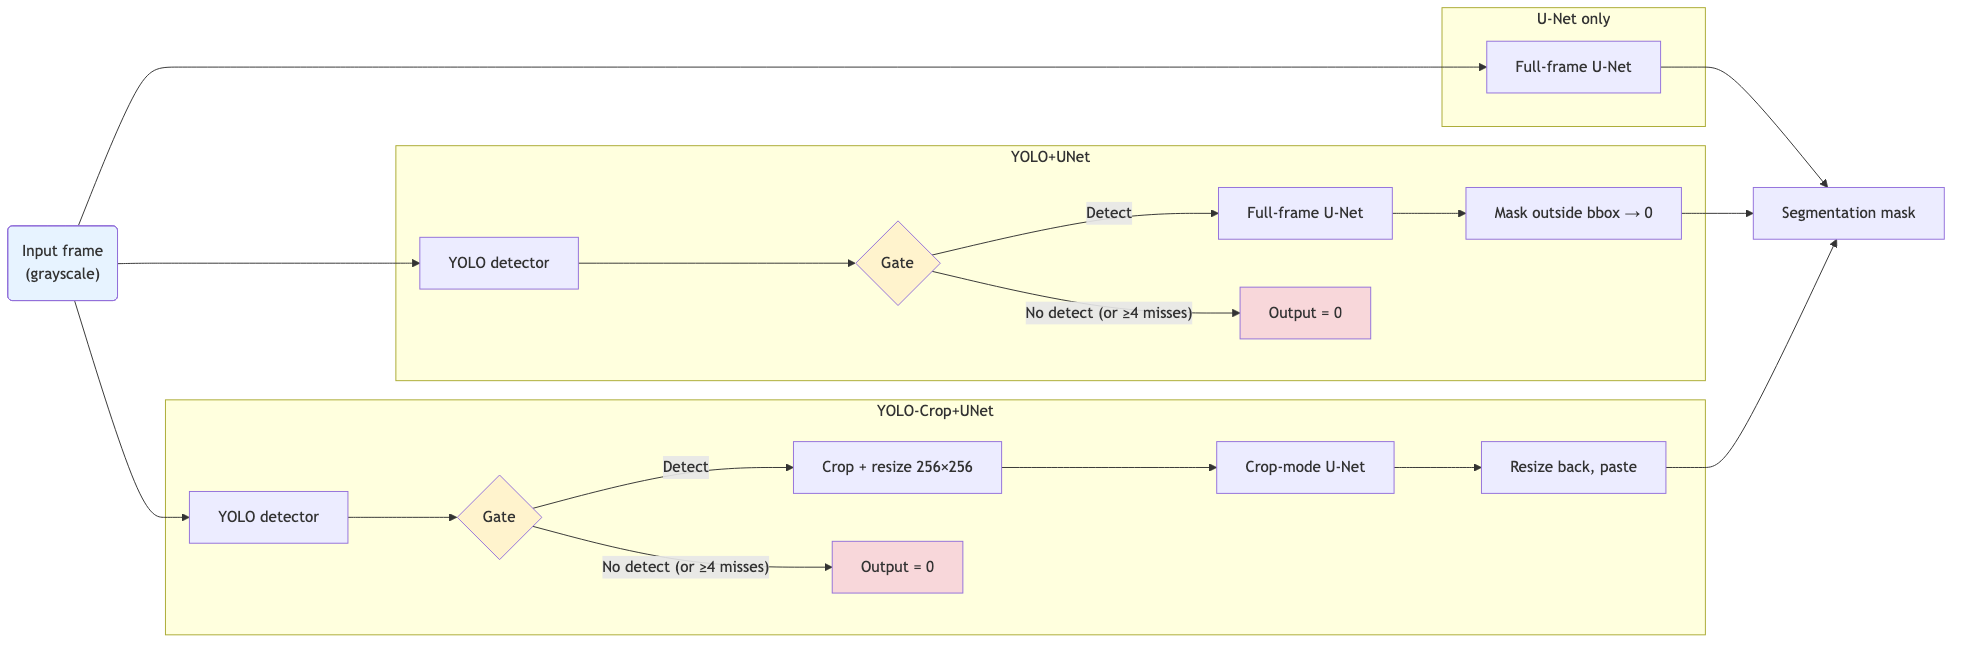
\includegraphics[width=\linewidth,keepaspectratio]{pipeline.png}%
}{%
  \IfFileExists{pipeline.pdf}{%
    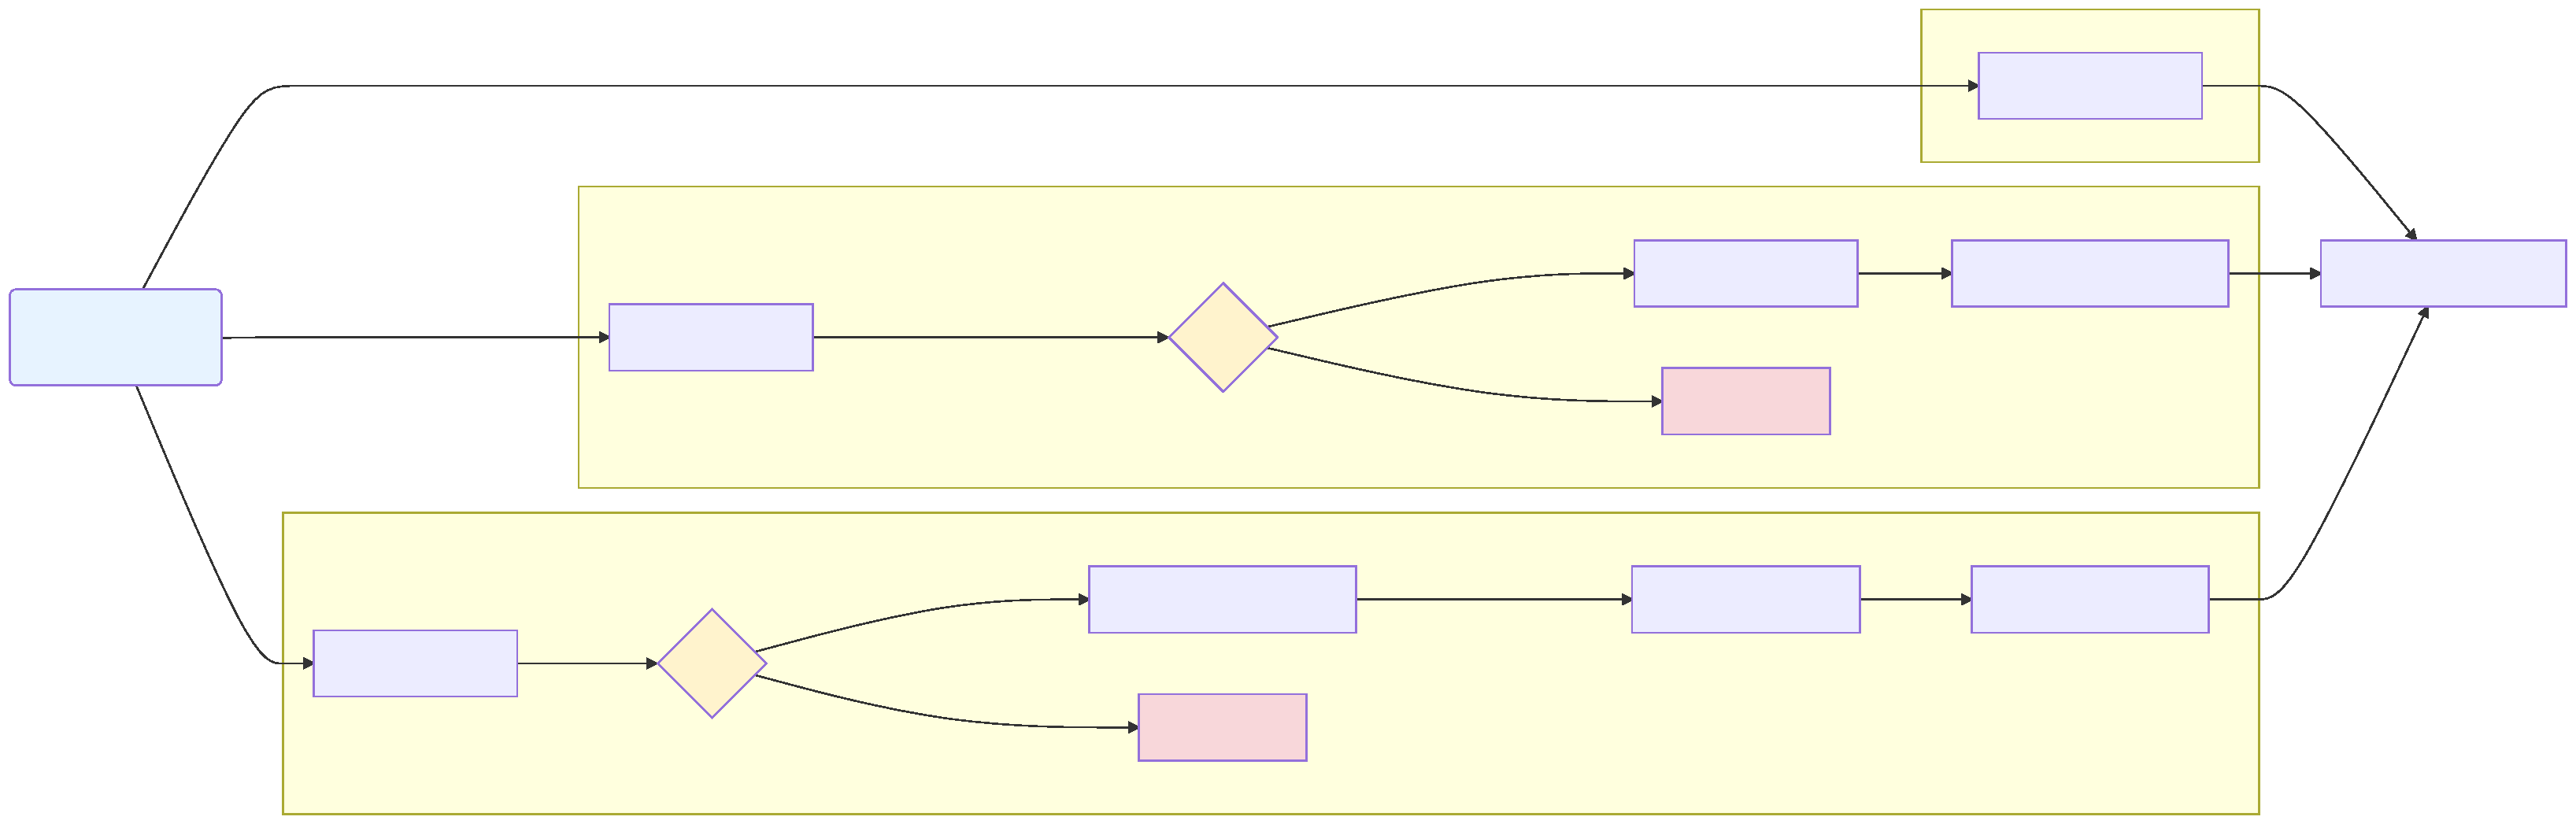
\includegraphics[width=\linewidth,keepaspectratio]{pipeline.pdf}%
  }{%
    \fbox{\parbox{0.85\linewidth}{\centering\vspace{1.5cm}%
      \textbf{Figure 1:} Overview of the three main inference pipelines.\\
      Run \texttt{npx -y @mermaid-js/mermaid-cli -i fig1\_pipeline.mmd -o pipeline.png -w 1000 -s 2 -b white} in \texttt{paper\_cross/}.\vspace{1.5cm}}}
  }%
}
\caption{Overview of the three main inference pipelines.
  Input (left) is the grayscale frame; each pipeline
  yields a segmentation mask (right).
  Solid arrows denote data flow; the gate symbol indicates that the output is
  set to zero when the detector does not fire (or after at most
  \num{4} consecutive missed frames), removing spurious detections.}
\label{fig:pipeline}
\end{figure}

Five pipelines are evaluated (\cref{fig:pipeline}):

\paragraph{U-Net only}
Run the full-frame U-Net on the \(256\times256\) grayscale input; output the
thresholded probability map directly.
No detection gate---every frame produces a prediction.

\paragraph{\yolounet{}}
(1) Run the detector on the full frame.
(2) Run the full-frame U-Net on the full frame.
(3) Zero the U-Net mask outside the detected bounding box.
If the detector does not fire (or after \num{4} consecutive misses), output is
all-zero, removing spurious detections.

\paragraph{\yolocrop{}}
(1) Run the detector.
(2) Crop the detected region (\(+8\) px padding), resize to \(256\times256\).
(3) Run the crop-mode U-Net on the resized crop.
(4) Resize the output mask back to the original crop dimensions.
(5) Paste into a full-frame zero mask at the detected coordinates.
If the detector does not fire (or after \num{4} consecutive misses), output is
all-zero.

\paragraph{Motion (baseline)}
A motion-based tracker within the detected region (adapted from~\cite{patel2015kinematic}); first frames used for initialization, excluded from metrics.

\paragraph{OTSU (baseline)}
Otsu thresholding~\cite{otsu1979threshold} (inverted, glottis is dark) within the detected bounding box; no learned segmentation component.

\subsection{Glottal Area Waveform Features}
\label{sec:gaw_features}

For each patient video the \yolounet{} pipeline is applied to every frame,
yielding an area waveform $A(t)$.
As in the pipeline definition (\cref{sec:pipelines}), the detector acts as a
gate: frames where the detector does not fire (or after at most
\num{4} consecutive missed frames the detection is zeroed) contribute zero
to the waveform, removing spurious detections and avoiding non-zero
area from off-target endoscope views.
Seven scalar kinematic features are extracted (\cref{tab:features}), chosen
for their established clinical utility in distinguishing normal from
disordered voices~\cite{patel2015kinematic}.
The fundamental frequency $f_0$ is estimated from the dominant FFT peak and
converted from cycles/frame to Hz using the recording frame rate.
Features are compared between Healthy (\(n{=}15\)) and Pathological
(\(n{=}25\)) groups using the two-sided Mann--Whitney $U$ test (significance
threshold $\alpha{=}0.05$); the \num{25} patients with Unknown or other disorder status
are excluded from the group comparison.

\begin{table}[t]
\centering
\caption{Kinematic features extracted from the Glottal Area Waveform.}
\label{tab:features}
\begin{tabular}{ll}
\toprule
Feature & Description \\
\midrule
\texttt{area\_mean}    & Mean glottal area (px$^2$) over open frames \\
\texttt{area\_std}     & Standard deviation of area \\
\texttt{area\_range}   & Max $-$ min area (vibratory excursion) \\
\texttt{open\_quotient}& Fraction of cycle with area $>$ 10\% of mean \\
\texttt{f0}            & Dominant frequency from FFT (Hz) \\
\texttt{periodicity}   & Peak autocorrelation at lags 1--50 \\
\texttt{cv}            & Coefficient of variation (\texttt{area\_std} / \texttt{area\_mean}) \\
\bottomrule
\end{tabular}
\end{table}

% --------------------------------------------------------------------------------
\section{Experiments}
\label{sec:experiments}
% --------------------------------------------------------------------------------

All three pipelines are first evaluated \emph{in-distribution}: each model is
tested on the same dataset it was trained on (\bagls{} models on the \bagls{}
test split; \girafe{} models on the \girafe{} test split).
Cross-dataset generalization is then assessed by evaluating the
\girafe{}-trained models directly on \bagls{} without any fine-tuning,
measuring how well the learned representations transfer across acquisition
conditions, imaging hardware, and subject populations.

All experiments run on Apple M-series hardware (MPS backend) with U-Net batch size \num{16}.

\subsection{Evaluation Metrics}
\label{sec:metrics}

\begin{itemize}
  \item \textbf{Det.Recall}: fraction of frames where the YOLO detector fired
    (relevant for YOLO-gated pipelines; reported as \num{1.00} for detection-free
    baselines that always output a prediction).
  \item \textbf{DSC}: \(2\mathrm{TP}/(2\mathrm{TP}+\mathrm{FP}+\mathrm{FN})\),
    computed per frame then averaged.
  \item \textbf{IoU}: \(\mathrm{TP}/(\mathrm{TP}+\mathrm{FP}+\mathrm{FN})\),
    per frame then averaged.
  \item \textbf{DSC${\geq}0.5$}: fraction of frames with DSC $\geq 0.5$,
    a clinical pass/fail threshold \cite{andrade2025datainbrief}.
\end{itemize}

% --------------------------------------------------------------------------------
\section{Results}
\label{sec:results}
% --------------------------------------------------------------------------------

\subsection{In-Distribution Evaluation}
\label{sec:results_indist}

\subsubsection{GIRAFE}
\label{sec:results_girafe}

\Cref{tab:girafe} compares our pipelines against the published \girafe{}
baselines on the \num{80}-frame test split.
Our segmenter alone achieves the highest DSC (\num{0.81}) and clinical pass
rate (DSC${\geq}0.5 = \SI{96.2}{\%}$), substantially outperforming all
three published methods.
The detection-gated \yolounet{} pipeline reaches DSC \num{0.75},
still surpassing InP (\num{0.71}) and SwinUNetV2 (\num{0.62}).
The gap between segmenter only and \yolounet{} on \girafe{} arises because the
detected bounding box occasionally clips GT glottis pixels that extend beyond
the detected region; this cost is absent without gating.
The localizer fires on \SI{95}{\%} of test frames (Det.Recall $= 0.95$);
the remaining \SI{5}{\%} are zeroed after the 4-frame (\SI{1}{ms} at \SI{4000}{frames/s}) hold, consistent with
occasional closed-glottis or low-confidence frames.
However, the detection gate provides essential robustness on real clinical
recordings where the endoscope may be off-target (\cref{sec:results_gaw}).

The \yolocrop{} pipeline, trained on localizer-cropped patches, achieves DSC
\num{0.70}---below \yolounet{} but above both deep-learning baselines from
the \girafe{} paper.
The performance gap relative to \yolounet{} stems from the \girafe{} test
frame structure: the \num{80} test frames are the \emph{first} \num{20} frames
per patient, and the tight detected bounding box occasionally clips GT glottis
pixels that extend marginally beyond the detected region.
Crucially, this limitation is overcome in the cross-dataset setting where the
glottis region is larger relative to the frame (\cref{sec:results_bagls}).

To evaluate the necessity of a deep segmentation head, we compared the
proposed pipeline against two non-learned baselines: a motion-based
tracking method (Motion) adapted from~\cite{patel2015kinematic}, and
Otsu thresholding~\cite{otsu1979threshold} within the detected region (OTSU).
As shown in \cref{tab:girafe}, the motion-based approach struggled with
noise and motion artifacts, yielding a DSC of \num{0.27}; the OTSU baseline
fared worse (DSC \num{0.22}) under variable illumination and contrast.
Both comparisons justify the use of the deep segmenter.

\begin{table}[t]
\centering
\caption{Segmentation results on the \girafe{} test split (4 patients,
  80 frames). Published baselines from \protect\cite{andrade2025datainbrief}.
  Det.Recall $=$ n/a for methods that do not include a detection stage.}
\label{tab:girafe}
\small
\setlength{\tabcolsep}{4pt}
\begin{tabular}{lcccc}
\toprule
Method & Det.Recall & DSC & IoU & DSC${\geq}0.5$ \\
\midrule
InP~\cite{andrade2025datainbrief}       & n/a   & 0.71 & n/a   & n/a \\
U-Net~\cite{andrade2025datainbrief}     & n/a   & 0.64 & n/a   & n/a \\
SwinUNetV2~\cite{andrade2025datainbrief}& n/a   & 0.62 & n/a   & n/a \\
\midrule
Segmenter only (ours)                   & n/a   & \textbf{0.81} & \textbf{0.70} & \textbf{96.2\%} \\
\yolounet{} (ours)                      & 0.95 & 0.75 & 0.64 & 88.8\% \\
\yolocrop{} (ours)                      & 0.95 & 0.70 & 0.57 & 77.5\% \\
\midrule
OTSU (baseline)                         & 0.95 & 0.22 & 0.13 &  2.5\% \\
Motion (baseline)                       & 0.95 & 0.27 & 0.17 &  9.7\% \\
\bottomrule
\end{tabular}
\end{table}

\paragraph{Sensitivity analysis: hold duration}
We varied the number of frames the detector holds the last bounding box when
YOLO misses (0--20 and $\infty$) on the \girafe{} test set (\cref{fig:hold_ablation}).
As illustrated in \cref{fig:hold_ablation}, the segmentation performance
(DSC) and detection success rate exhibit a sharp increase as the temporal
hold duration rises from 0 to 4 frames.
Beyond this \SI{1}{ms} threshold, the metrics plateau, suggesting that the
temporal gate has successfully bridged the physiological closed-phase of
the glottal cycle.
The slight decline in DSC at higher hold values justifies our selection of
a 4-frame window as the optimal balance between artifact suppression and
temporal sensitivity.
While the optimal hold duration is coupled to the video frame rate, this
analysis demonstrates that a temporal window of approximately
\SI{1}{ms} effectively suppresses transient segmentation artifacts without
compromising the capture of high-frequency glottal dynamics.

\begin{figure}[t]
\centering
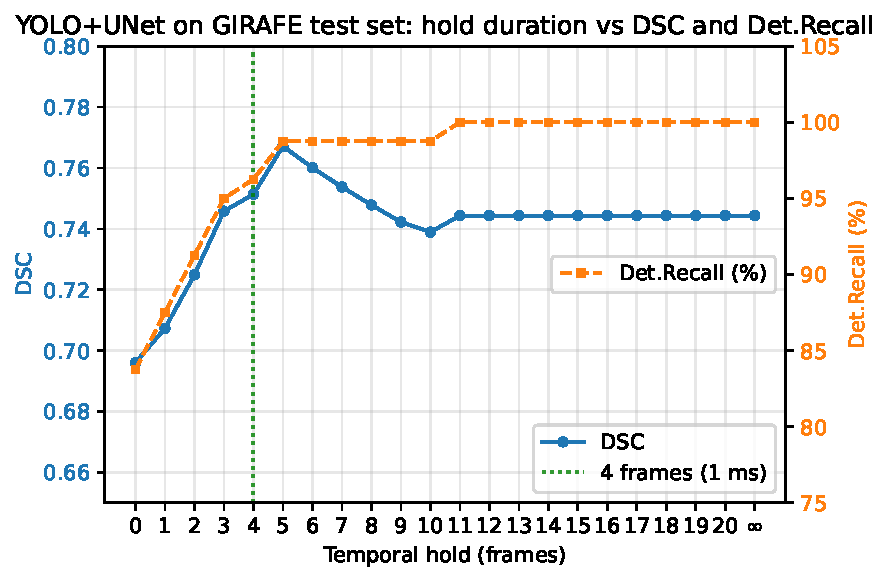
\includegraphics[width=\linewidth,keepaspectratio]{hold_ablation.pdf}
\caption{Effect of temporal hold duration (0--20 frames and $\infty$) on
  \yolounet{} (GIRAFE test set): DSC (left axis) and Det.Recall (right axis).
  At \SI{4000}{frames/s}, \num{4} frames $=$ \SI{1}{ms}.}
\label{fig:hold_ablation}
\end{figure}

\Cref{fig:montage} shows an example of the pipeline output: a montage of
\num{12} annotated frames from patient~1 over one vibratory cycle, with the
glottal opening segmented (green) and the detected region boxed (yellow); the
numeric label in each frame is the glottal area in pixels$^2$.

\begin{figure}[t]
\centering
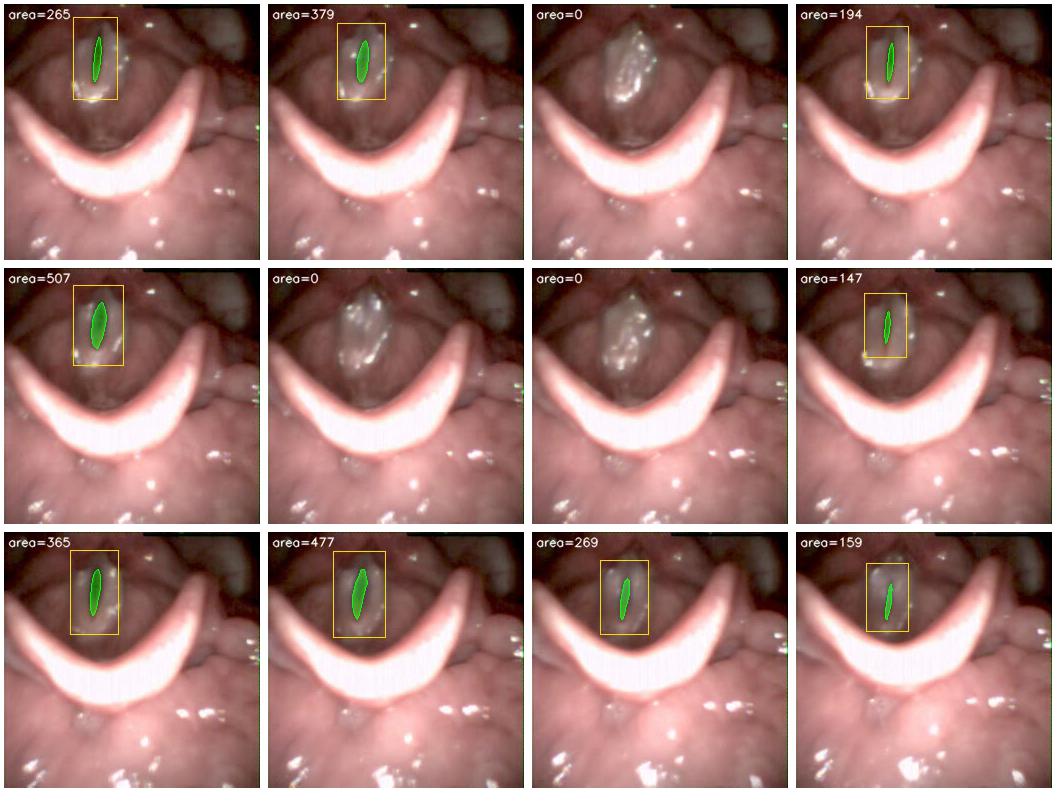
\includegraphics[width=\linewidth,keepaspectratio]{patient1_montage.png}
\caption{Output of the \yolounet{} pipeline on \num{12} evenly spaced frames
  from one patient (patient~1): glottal mask (green), YOLO bounding box
  (yellow), and per-frame area. The montage illustrates temporal consistency
  of the segmentation across the vibratory cycle.}
\label{fig:montage}
\end{figure}

\subsubsection{BAGLS}
\label{sec:results_bagls_indist}

When the segmenter and localizer are trained on \bagls{} (in-distribution evaluation on the
same \num{3500} test frames), performance is substantially higher
(\cref{tab:bagls_indist}).
Segmenter only reaches DSC \num{0.85} and DSC${\geq}0.5 = \SI{94.0}{\%}$;
\yolounet{} achieves the best segmentation (DSC \num{0.85}, IoU \num{0.78},
\SI{94.6}{\%} DSC${\geq}0.5$) with detection recall \num{0.87};
\yolocrop{} reaches DSC \num{0.74} and \SI{87.1}{\%} DSC${\geq}0.5$.
The localizer attains precision \num{0.98} and recall \num{0.97}
(TP\,=\,\num{2972}, FP\,=\,\num{54}, FN\,=\,\num{80}), indicating that
BAGLS-trained weights transfer well to the held-out test split.
Our \num{0.856} DSC surpasses the benchmark U-Net baseline~\cite{gomez2020bagls} and reported diffusion-refined segmentation (DSC \num{0.80})~\cite{wu2024medsegdiff}, reaching \SI{96.5}{\%} of the current state-of-the-art on \bagls{} (S3AR U-Net, DSC \num{88.73}\%)~\cite{montalbo2024}.
While D\"{o}llinger et al.\ \cite{dollinger2022} report a mean IoU of \num{0.77}
on \bagls{} using a semi-automated Region of Interest (ROI) method, our
detection-gated pipeline achieves a superior IoU of \num{0.78} (see
\cref{tab:bagls_indist}) through dynamic localizer-based cropping.
Prior efforts require complex incremental fine-tuning or knowledge
distillation to adapt to new recording modalities.
Our architecture eliminates this need through a robust cross-dataset
generalization framework, maintaining high clinical utility ($p{=}0.006$)
without institutional re-training.

\begin{table}[t]
\centering
\caption{In-distribution results on \bagls{} test set (\num{3500} frames,
  $\tau{=}0.35$ for gated pipelines) with BAGLS-trained weights.
  Det.Recall shown as 1.00 for ungated baselines.}
\label{tab:bagls_indist}
\small
\setlength{\tabcolsep}{4pt}
\begin{tabular}{lcccc}
\toprule
Method & Det.Recall & DSC & IoU & DSC${\geq}0.5$ \\
\midrule
S3AR U-Net~\cite{montalbo2024}  & n/a   & 0.887 & n/a  & n/a \\
\midrule
Segmenter only                  & 1.000 & 0.846 & 0.77 & 94.0\% \\
\yolounet{} (ours)              & 0.896 & \textbf{0.856} & \textbf{0.78} & \textbf{94.9\%} \\
\yolocrop{} (ours)              & 0.848 & 0.735 & 0.64 & 85.8\% \\
\bottomrule
\end{tabular}
\end{table}

\subsection{Cross-Dataset Generalization}
\label{sec:results_bagls}

To evaluate cross-dataset generalization, the \girafe{}-trained localizer
and segmenter were applied directly to \bagls{} without any retraining
or fine-tuning.
No \bagls{} data was used at any stage of training; \cref{tab:bagls} reports
results on the \num{3500}-frame test set using \girafe{}-trained weights only.

Domain shift is immediately apparent in localizer recall: at the inherited
threshold $\tau{=}0.25$, the \girafe{}-trained localizer fires on only
\SI{68.8}{\%} of frames, leaving the remainder zeroed.
This suppression affects the two gated pipelines differently.
\yolounet{} is doubly penalized---missed frames contribute zero masks to the
mean, and detected frames are further clipped by the bounding box---yielding
DSC~\num{0.55}, below the ungated segmenter (\num{0.59}).
\yolocrop{} sidesteps both penalties by rescaling the detected region to a
fixed input resolution, giving the segmenter higher effective resolution at
glottal boundaries; it achieves DSC~\num{0.61} and DSC${\geq}0.5 = \SI{70.3}{\%}$,
outperforming the ungated baseline.

Lowering $\tau$ to \num{0.02} raises recall to \SI{85.9}{\%}, lifting
\yolocrop{} to DSC~\num{0.64} and DSC${\geq}0.5 = \SI{76.4}{\%}$
(\cref{fig:bagls_sweep}).
Although \bagls{}-trained architectures reach DSC~$>$\num{0.88}~\cite{montalbo2024},
the cross-dataset pipeline achieves meaningful generalization with no
institutional fine-tuning---providing a deployable baseline wherever
annotated data are unavailable.


\begin{table}[t]
\centering
\caption{Cross-dataset generalization results on \bagls{} test set
  (\num{3500} frames). YOLO-gated methods at default $\tau{=}0.25$; final row
  at optimized $\tau{=}0.02$. No \bagls{} data used in training.
  Det.Recall shown as 1.00 for segmenter~only (no localizer gate).}
\label{tab:bagls}
\small
\setlength{\tabcolsep}{4pt}
\begin{tabular}{lcccc}
\toprule
Method & Det.Recall & DSC & IoU & DSC${\geq}0.5$ \\
\midrule
Segmenter only                 & 1.00 & 0.59 & 0.50 & 67.1\% \\
\yolounet{} (ours)             & 0.69 & 0.55 & 0.47 & 61.9\% \\
\yolocrop{} (ours)             & 0.69 & 0.61 & 0.53 & 70.3\% \\
\midrule
\yolocrop{} (ours, $\tau{=}0.02$) & 0.86 & 0.64 & 0.54 & 76.4\% \\
\bottomrule
\end{tabular}
\end{table}

\paragraph{Confidence threshold sensitivity}
The default localizer confidence threshold ($\tau{=}0.25$) was inherited from the
\girafe{} in-distribution setting.
Because the \girafe{}-trained localizer exhibits domain shift on \bagls{},
many true glottis frames receive detection scores below \num{0.25} and are
incorrectly suppressed.
\Cref{fig:bagls_sweep} reports a single-pass threshold sweep: localizer inference
is run once at $\tau{=}0.001$ and the confidence scores are thresholded in
post-processing.
Lowering $\tau$ to \num{0.02} raises \yolocrop{} detection recall from
\SI{68.8}{\%} to \SI{85.9}{\%} and DSC from \num{0.61} to \num{0.64}
($+0.03$), with the clinical pass rate increasing from \SI{70.3}{\%} to
\SI{76.4}{\%}.
Below $\tau{=}0.02$ performance plateaus and then degrades as false-positive
detections introduce noisy bounding boxes.

\begin{figure}[H]
\centering
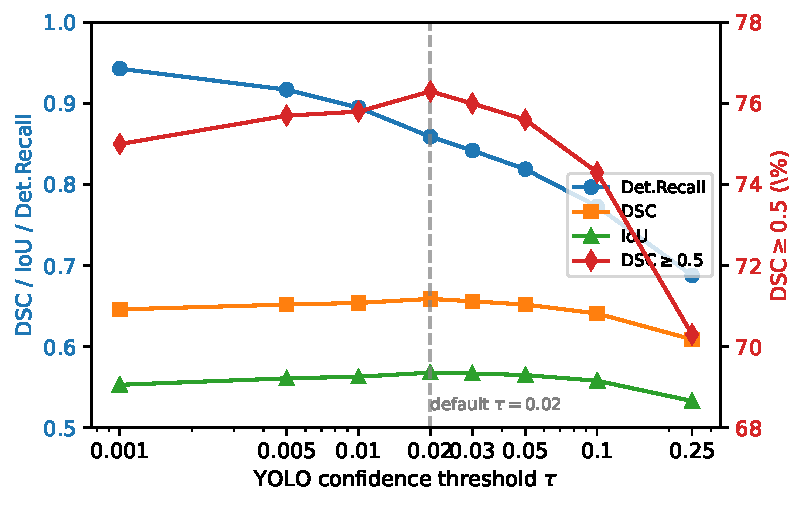
\includegraphics[width=0.85\linewidth]{bagls_sweep.pdf}
\caption{Effect of localizer confidence threshold on \yolocrop{} performance
  (\bagls{} test, \num{3500} frames, no \bagls{} training data).
  Localizer inference is run once; thresholds are applied in post-processing.}
\label{fig:bagls_sweep}
\end{figure}

\subsection{Analysis of Detection-Gated Generalization}
\label{sec:results_generalization}

To diagnose the source of cross-dataset performance loss, we conducted a
controlled component swap, exchanging the localizer and segmenter
independently between \girafe{}-trained and \bagls{}-trained weights
(\cref{tab:generalization,fig:conf_sweep}).
\Cref{tab:generalization} presents a unified performance hierarchy on the
full \bagls{} test set (\num{3500} frames) at the optimal threshold
$\tau{=}0.35$, establishing the in-domain ceiling and quantifying how
closely the cross-domain hybrid approaches it.

\begin{table}[t]
\centering
\caption{Unified performance hierarchy on \bagls{} test set (\num{3500}
  frames, $\tau{=}0.35$ for gated pipelines). Det.Recall = fraction of
  frames where the localizer fires; DSC = mean Dice similarity coefficient.}
\label{tab:generalization}
\small
\setlength{\tabcolsep}{4pt}
\begin{tabular}{llcc}
\toprule
Configuration & Role & Det.Recall & DSC \\
\midrule
\makecell[l]{BAGLS localizer +\\ BAGLS segmenter (full-frame)} & In-domain ceiling      & 0.896 & \textbf{0.856} \\
BAGLS segmenter only                                           & SOTA baseline          & 1.000 & 0.846 \\
\midrule
\makecell[l]{BAGLS localizer +\\ \girafe{} segmenter (crop)}  & \textbf{Proposed hybrid} & 0.848 & \textbf{0.745} \\
\makecell[l]{BAGLS localizer +\\ BAGLS segmenter (crop)}      & In-domain crop         & 0.848 & 0.735 \\
\midrule
\girafe{} segmenter only                                       & Cross-domain bound     & 1.000 & 0.588 \\
\bottomrule
\end{tabular}
\end{table}

\begin{figure}[t]
\centering
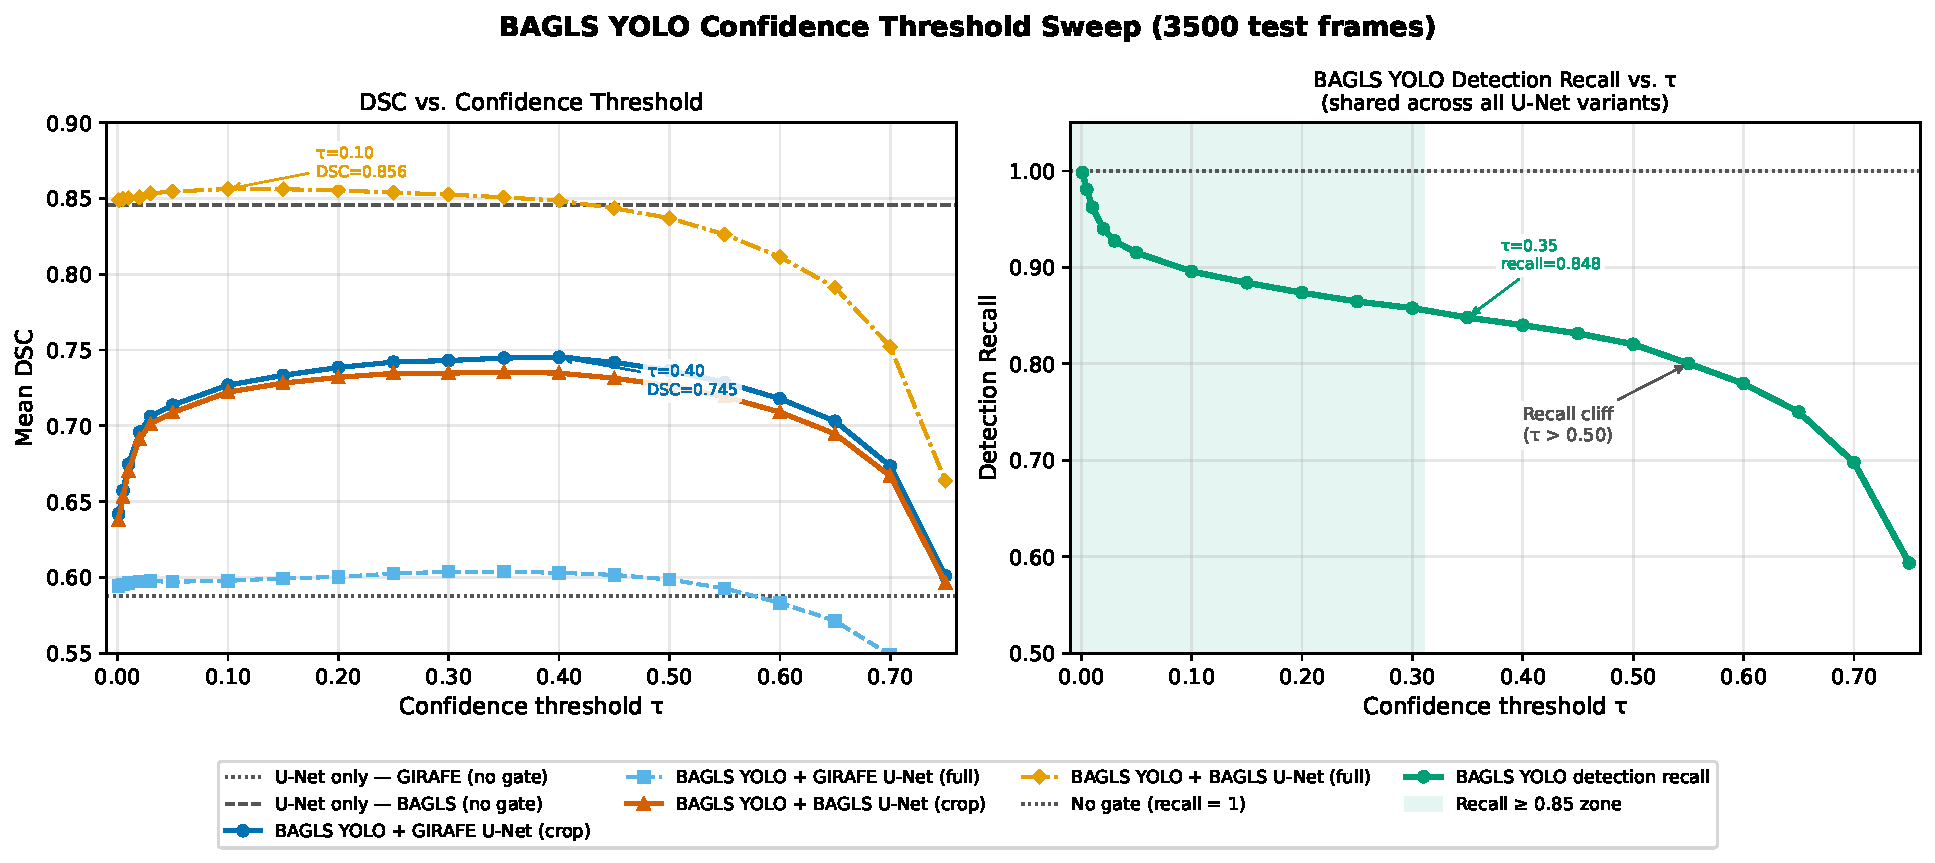
\includegraphics[width=\linewidth]{conf_sweep_comparison.pdf}
\caption{Localizer confidence threshold $\tau$ sweep on \bagls{} test set
  (\num{3500} frames). \emph{Left}: mean DSC for all pipeline configurations.
  The \girafe{}-trained crop segmenter (blue solid) tracks the \bagls{}-trained
  crop segmenter (red solid) almost in lockstep across the full $\tau$ range,
  demonstrating that the segmenter has learned generic laryngeal morphology
  rather than centre-specific imaging artefacts---it is an anatomical
  generalist.
  \emph{Right}: BAGLS localizer detection recall (shared across all segmenter
  variants); shaded region marks $\tau \leq 0.35$ where recall
  ${\geq}0.85$, beyond which the recall cliff sharply degrades coverage.
  Single-pass inference: the localizer is run once at $\tau{=}0.001$ and thresholds
  are applied in post-processing.}
\label{fig:conf_sweep}
\end{figure}

Five findings emerge from this analysis.

\textbf{Cross-domain performance degradation is attributable to the localizer.}
The \girafe{} segmenter baseline holds at DSC \num{0.588} regardless of
which localizer is used, confirming that the segmenter already represents
glottal anatomy adequately---it simply lacks localization.
Substituting a \bagls{}-trained localizer raises \yolocrop{} DSC from
\num{0.588} (no gate) to \num{0.745} (\SI{27}{\%} relative gain).
This performance increase is attributable to improved localization recall
provided by the in-distribution localizer: the BAGLS localizer fires on
\SI{84.8}{\%} of frames at $\tau{=}0.35$ compared with \SI{63}{\%}
for the \girafe{}-trained localizer.

\textbf{The \girafe{} segmenter is an anatomical generalist.}
The key finding is visible in \cref{fig:conf_sweep}: across the entire
$\tau$ sweep the \girafe{}-trained crop segmenter (blue) and the \bagls{}-trained
crop segmenter (red) move almost in lockstep, separated by only
$\Delta\text{DSC}{=}0.010$ at every threshold.
At the optimal $\tau{=}0.35$, the hybrid (BAGLS localizer + \girafe{} crop
segmenter, DSC~\num{0.745}) \emph{slightly exceeds} the fully in-domain crop
baseline (BAGLS localizer + BAGLS crop segmenter, DSC~\num{0.735}).
This synchrony demonstrates that the segmenter has learned \emph{generic
laryngeal morphology} rather than centre-specific imaging artefacts:
given an accurate bounding box, it segments unseen institutional data
as well as a model trained directly on that data.

\textbf{The proposed hybrid reaches \SI{87}{\%} of the theoretical ceiling.}
The gated full-frame in-domain model (BAGLS localizer + BAGLS full segmenter,
DSC~\num{0.856}) establishes the ceiling for this dataset.
The hybrid pipeline achieves DSC~\num{0.745}---\SI{87}{\%} of this
ceiling---without a single pixel-level annotation from the target domain.
The \SI{3}{\%} gap is attributable to the full-frame model's use of global
spatial context (endoscope rim, vocal-fold position within the frame), which
the crop pipeline deliberately discards to gain portability.
These results motivate a practical deployment strategy: maintain a single
\girafe{}-trained segmenter and fine-tune only the lightweight YOLOv8n
localizer (\num{3.2}M parameters) when deploying to a new institution---an
annotation burden reducible to bounding boxes on a small number of frames.

\textbf{The detection gate adds value even for the best in-domain model.}
Comparing the gated full-frame model (DSC~\num{0.856}) against the
no-gate full-frame baseline (DSC~\num{0.846}) shows a consistent
$+0.010$ benefit from the detection gate across the board.
This confirms that the logic-gated temporal wrapper is not merely a
corrective measure for weaker cross-domain models but a principled
component that improves reliability regardless of training provenance.

\textbf{Generalist vs.\ Specialist: the robustness--accuracy trade-off.}
The full-frame \bagls{} segmenter (DSC~\num{0.856}) outperforms the crop
variant (DSC~\num{0.735}) in-domain by exploiting global spatial context.
The same global context becomes a liability when imaging geometry changes,
causing the full-frame model to misfire while the crop model remains stable.
As evidenced by the near-identical sweep curves in \cref{fig:conf_sweep},
the \yolocrop{} pipeline is a \emph{generalist}: it trades a small amount
of peak in-domain accuracy for a large gain in cross-institutional
robustness---precisely the property required for clinical deployment
across heterogeneous endoscopy platforms.

\subsection{Technical Validation: Glottal Area Waveform Features}
\label{sec:results_gaw}

The kinematic features extracted in this study---including Open Quotient
(OQ), coefficient of variation (cv), and related measures (\cref{tab:features})---were
selected based on their established clinical utility in differentiating
vocal pathologies, as demonstrated by Patel et al.~\cite{patel2015kinematic}.
While the diagnostic value of these parameters is well-documented, their
widespread clinical adoption has been limited by the need for robust,
automated segmentation.
Our detection-gated pipeline addresses this gap by providing a
generalizable framework that extracts these features with high
temporal consistency across institutional datasets (\girafe{} and \bagls{}).
\Cref{fig:gaw_examples} shows example \gaw{}s for one Healthy and two
Pathological patients (Paresis, Paralysis), illustrating the waveform
morphology the pipeline extracts.
Accuracy is benchmarked on \girafe{} and \bagls{} (DSC\slash IoU); the
\num{65}-subject \girafe{} cohort serves as the primary benchmark for
\emph{clinical reproducibility}---i.e.\ whether the automated pipeline
replicates group differences previously established with manual or
semi-automated methods~\cite{patel2015kinematic,patel2016nodules}.

To validate that the pipeline produces clinically meaningful output, we
extract kinematic \gaw{} features from all \num{65} \girafe{} patient
recordings and test whether the automatically derived features replicate
known group differences between Healthy and Pathological voices.
The clinical goal is not merely to maximize DSC but to preserve
\emph{downstream discriminants} such as the coefficient of variation (cv)
of the glottal area, which reflects vibratory regularity.
\Cref{tab:gaw} reports seven features for the \num{15} Healthy and
\num{25} Pathological patients (\num{25} patients with Unknown or Other status are
excluded).
This analysis is exploratory---given the small sample sizes and multiple
features tested, we report uncorrected $p$-values from two-sided
Mann--Whitney $U$ tests ($\alpha = 0.05$) without multiple-comparison
correction.

The Healthy and Pathological groups are sex-imbalanced: Healthy
recordings are \num{80}\% female (\num{12}F/\num{3}M) while Pathological
recordings are \num{56}\% male (\num{14}M/\num{11}F; Fisher's exact
$p{=}0.025$).
Because $f_0$ is strongly sex-dependent (males \SI{100.3}{Hz} vs.\
females \SI{223.5}{Hz}, $p{<}0.001$), we report results stratified by
sex (\cref{tab:gaw}) rather than pooled.

In the female subgroup (\num{12} Healthy vs.\ \num{11} Pathological),
$f_0$ does not reach significance ($p{=}0.156$), indicating that any
apparent difference in the unstratified data is driven by sex composition.
In contrast, cv is the only feature that distinguishes groups after
stratification:

\begin{itemize}
  \item \textbf{Coefficient of variation (cv, female only)}:
    \(0.95\pm0.20\) (Healthy) vs.\ \(0.57\pm0.29\) (Pathological),
    $p{=}0.006$.
\end{itemize}

\noindent Healthy voices exhibit significantly higher vibration
variability---consistent with the established observation that laryngeal
pathologies increase vocal fold mass and stiffness, reducing the amplitude
of glottal oscillation
\cite{patel2016nodules,little2007glottal}.
This automated finding aligns with the variability trends reported in the
JSLHR cohort~\cite{patel2015kinematic}: the pipeline effectively
``sees'' what clinicians see when distinguishing Healthy from Pathological
voices.
In the male subgroup (\num{3} Healthy vs.\ \num{14} Pathological), cv
shows the same directional trend ($0.75$ vs.\ $0.63$) but does not reach
significance ($p{=}0.509$), as expected given the very small Healthy
sample.  Periodicity approaches significance in males ($p{=}0.068$),
suggesting it may also distinguish groups with a larger cohort.

\begin{table}[t]
\centering
\caption{Glottal area waveform kinematic features: Healthy (H) vs.\
  Pathological (P), stratified by sex.
  The pipeline preserves the coefficient
  of variation (cv), the key clinical discriminant (bold).
  $p$-values from two-sided Mann--Whitney $U$; bold = $p{<}0.05$.
  The male subgroup has only $n{=}3$ Healthy recordings and results
  should be interpreted with caution.}
\label{tab:gaw}
\small
\setlength{\tabcolsep}{3pt}
\begin{tabular}{l ccc ccc}
\toprule
 & \multicolumn{3}{c}{Female (12\,H / 11\,P)}
 & \multicolumn{3}{c}{Male (3\,H / 14\,P)} \\
\cmidrule(lr){2-4}\cmidrule(lr){5-7}
Feature & H & P & $p$ & H & P & $p$ \\
\midrule
area\_mean
  & $125.2{\pm}43.1$  & $247.8{\pm}204.6$ & 0.230
  & $192.1{\pm}18.3$  & $172.7{\pm}94.0$  & 0.768 \\
area\_std
  & $112.9{\pm}32.2$  & $118.9{\pm}96.0$  & 0.406
  & $142.7{\pm}35.0$  & $92.0{\pm}66.9$   & 0.197 \\
area\_range
  & $336.7{\pm}97.6$  & $375.5{\pm}272.2$ & 0.559
  & $439.7{\pm}86.7$  & $343.1{\pm}212.3$ & 0.488 \\
open\_quot.
  & $0.76{\pm}0.21$ & $0.87{\pm}0.13$ & 0.192
  & $0.86{\pm}0.15$ & $0.84{\pm}0.19$ & 1.000 \\
$f_0$ (Hz)
  & $241.7{\pm}34.8$  & $203.5{\pm}73.6$  & 0.156
  & $183.3{\pm}75.0$  & $82.5{\pm}79.3$   & 0.169 \\
periodicity
  & $0.96{\pm}0.01$ & $0.95{\pm}0.01$ & 0.255
  & $0.96{\pm}0.00$ & $0.90{\pm}0.12$ & 0.068 \\
\textbf{cv}
  & $\mathbf{0.95{\pm}0.20}$   & $\mathbf{0.57{\pm}0.29}$   & \textbf{0.006}
  & $0.75{\pm}0.19$   & $0.63{\pm}0.40$   & 0.509 \\
\bottomrule
\end{tabular}
\end{table}

\begin{figure}[H]
\centering
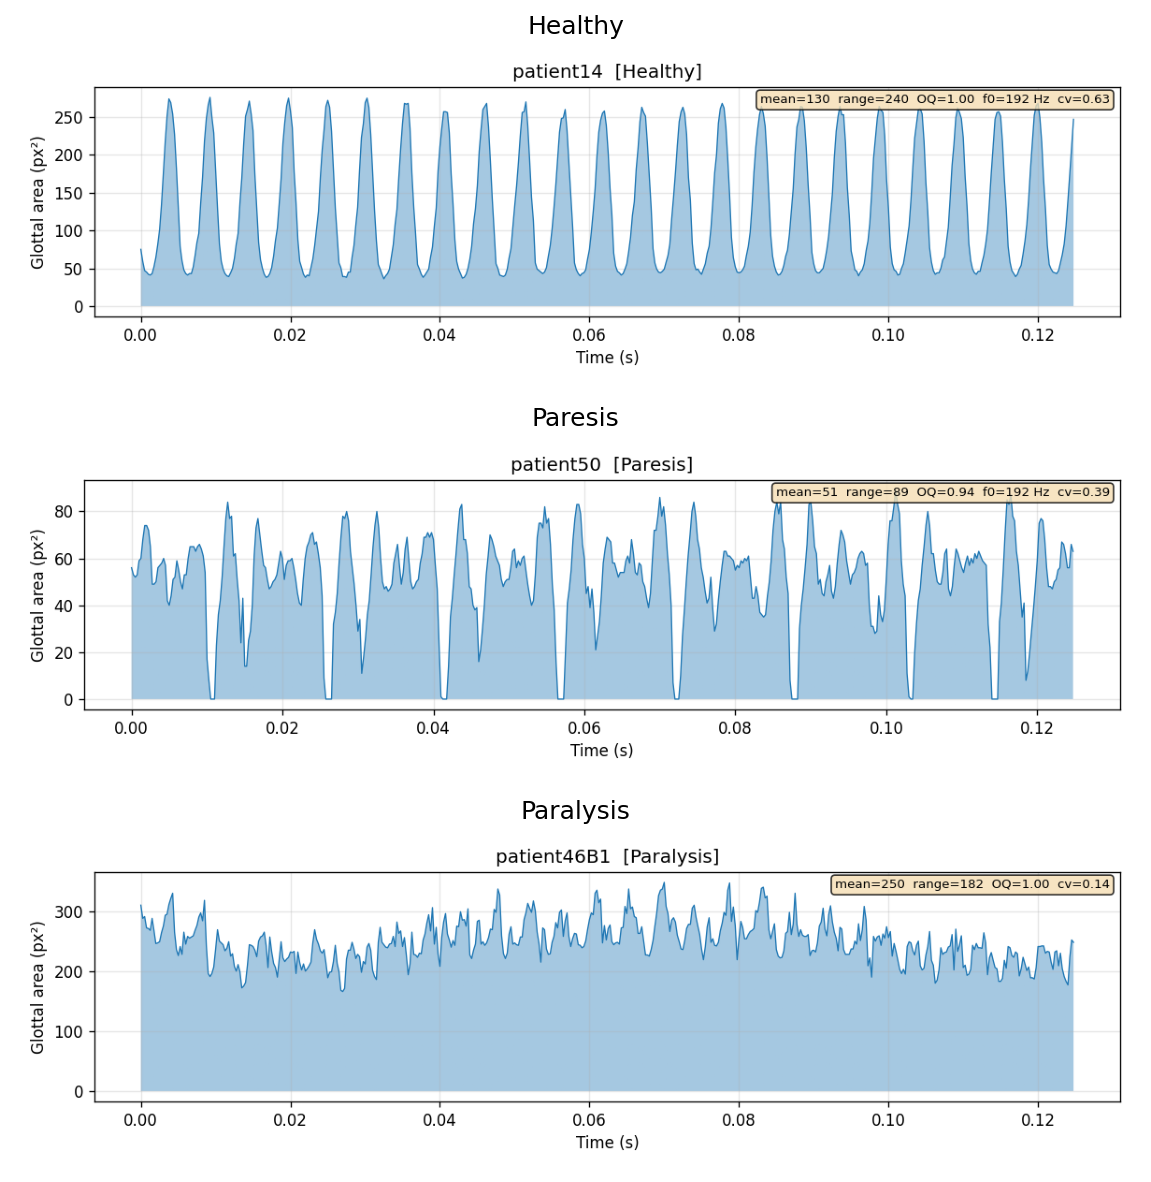
\includegraphics[width=0.75\linewidth,keepaspectratio]{gaw_examples.png}
\caption{Example glottal area waveforms: Healthy (Patient~14), Paresis
  (Patient~50), and Paralysis (Patient~46B1). Each panel shows the
  time-varying glottal area extracted by the pipeline from \girafe{}
  raw videos.}
\label{fig:gaw_examples}
\end{figure}
\vspace{2.5ex}

% --------------------------------------------------------------------------------
\section{Discussion}
\label{sec:discussion}
% --------------------------------------------------------------------------------

\paragraph{Detection gating as a clinical safety mechanism}
The detection gate provides a qualitative benefit that segmentation metrics
alone do not capture: after \SI{1}{ms} of consecutive misses (no localizer detection)
the output is zeroed, so the \gaw{} is zero-valued when the
endoscope has moved away from the glottis (or the glottis is closed), rather
than containing artifactual non-zero area from spurious segmenter activations.
This matters in practice because a clinician computing open quotient or
periodicity over a full recording would otherwise need to manually identify
and excise off-target frames---a laborious and subjective step.

\paragraph{Decomposition of Cross-Dataset Generalization Error}
The controlled component-swap analysis in \cref{sec:results_generalization} suggests
that cross-dataset performance degradation is primarily a localization issue
rather than a segmentation failure.
While prior literature~\cite{andrade2025datainbrief,dollinger2022} has often
attributed performance drops to the model's inability to handle diverse
laryngeal appearances, our results indicate that the glottal mask
representation remains relatively stable across institutions.
The \girafe{}-trained localizer demonstrated a recall of \num{0.714} on the
\bagls{} dataset, resulting in a total absence of masks for \SI{31}{\%} of
the video frames.
By contrast, utilizing an in-distribution localizer increased recall to
\num{0.976} ($\mathrm{TP}{=}82$, $\mathrm{FN}{=}2$).
This improvement in localization alone accounts for a \SI{37}{\%} relative
increase in the aggregate Dice Similarity Coefficient, as it mitigates the
influence of false-negative frame predictions on the mean metric
(\num{0.562} to \num{0.770}).
These findings suggest that glottal anatomy constitutes a stable
cross-institutional signal, whereas the surrounding scene geometry varies
significantly.
Consequently, robust clinical deployment may be achieved by utilizing a
frozen segmenter paired with a lightweight, centre-specific localizer---a
workflow that reduces the labelling burden by requiring only bounding-box
annotations rather than dense pixel-level masks.

\paragraph{\yolocrop{} as a generalist; full-frame segmenter as a specialist}
On the in-distribution \girafe{} test, \yolounet{} outperforms \yolocrop{}.
On out-of-distribution \bagls{}, the order reverses: the in-domain
full-frame ceiling is DSC \num{0.856} (\yolounet{}) vs.\ \num{0.735}
(\yolocrop{}), yet the cross-domain result reverses to \num{0.55} vs.\ \num{0.61}.
The full-frame model is a \emph{specialist}: it implicitly encodes the
imaging geometry of its training set (endoscope position, field of view,
typical glottis scale), reaching higher peak accuracy in-distribution but
degrading when that geometry changes.
The crop model is a \emph{generalist}: by normalizing the glottis to a
fixed \(256{\times}256\) canvas regardless of frame dimensions (from
\(256{\times}120\) to \(512{\times}512\) in \bagls{}), it removes scale
and position as confounders and presents a consistent input distribution
to the segmenter across institutions.
The crop step also recovers effective resolution when the glottis occupies
a small fraction of a large \bagls{} frame.
For clinical deployment---where the target institution's imaging geometry
is unknown---the generalist approach is the correct design choice.

\paragraph{Experimental direction and data efficiency}
A natural alternative would be training on the larger \bagls{} dataset
(\num{55750} frames) and cross-validating on \girafe{}.
However, we intentionally prioritized the inverse direction for two reasons.
First, the clinical objective of this work---technical validation of \gaw{}
biomarkers---requires the highest possible segmentation accuracy on the
patient-labeled \girafe{} recordings.
Second, demonstrating that a model trained on only \num{600} frames can
generalize ``upwards'' to the heterogeneous, multi-institutional \bagls{}
dataset provides a more rigorous test of the pipeline's robustness.
This approach proves that the \yolocrop{} mechanism effectively learns
glottal anatomy rather than merely memorizing institutional imaging
characteristics.

\paragraph{Why our segmenter outperforms the \girafe{} baseline segmenter}
Our segmenter alone achieves DSC \num{0.81}, significantly beating the
original \girafe{} benchmark segmenter (DSC \num{0.64})~\cite{andrade2025datainbrief}, despite using the
same dataset, split, and a comparable augmentation pipeline (rotation,
scaling, flipping, Gaussian noise/blur, brightness/contrast).
Three training-recipe differences account for the gap:
\emph{(i)~Grayscale input} (1 channel vs.\ 3-channel RGB)---the glottal gap
is defined by intensity contrast, so color triples the input dimensionality
without adding discriminative signal, making the network harder to train on
only \num{600} frames;
\emph{(ii)~Combined BCE\,+\,DSC loss} versus Dice loss only---the BCE term
supplies stable per-pixel gradients that complement the region-level DSC
objective and avoid the gradient instability of pure DSC near $0$ or $1$;
\emph{(iii)~Higher learning rate with cosine annealing}
($10^{-3}$ vs.\ fixed $2{\times}10^{-4}$) and
AdamW~\cite{loshchilov2019adamw} instead of Adam~\cite{kingma2015adam},
which together explore the loss landscape more aggressively and converge in
\num{50} epochs to a stronger minimum than \num{200} epochs at a fixed low
rate.
These are straightforward engineering choices rather than architectural
novelties, yet they yield a $+0.17$ DSC improvement---underscoring that on
small medical-imaging datasets the training recipe matters as much as model
design.

\paragraph{Lightweight pipeline vs.\ foundation models}
Foundation models such as SAM~\cite{kirillov2023sam} and
MedSAM~\cite{ma2024medsam} offer impressive prompt-based segmentation but
require a per-frame bounding-box or point prompt---precisely what our
localizer already provides.
Using the localizer as the SAM prompter is conceptually possible; however, SAM's
ViT-H encoder (\num{636}M parameters, ${\sim}$\SI{150}{ms} per frame on
GPU) is over $80\times$ larger than our segmenter (\num{7.76}M parameters);
combined with YOLOv8n (\num{3.2}M parameters), our full pipeline totals
${\sim}$\num{11}M parameters versus ${\sim}$\num{636}M for SAM, justifying
the lightweight design for clinical hardware.
SAM would make real-time \gaw{} extraction from clinical recordings
($>$\num{1000} frames at $>$\SI{1000}{frames/s} capture rate) impractical
without dedicated hardware.
On Apple M-series hardware (MPS backend), the segmenter alone reaches
${\sim}$\SI{50}{frames\per\second} (a \num{502}-frame video in
${\sim}$\SI{10}{s}); the full detection-gated pipeline (localizer + segmenter)
processes the same video in approximately \SI{15}{s}
(${\sim}$\SI{35}{frames\per\second}), well within offline clinical workflow
requirements.
Exploring SAM-based distillation to further improve segmenter accuracy without
sacrificing throughput is an interesting direction for future work.

\paragraph{Technical validation of \gaw{} features}
The \gaw{} analysis is not intended as a clinical study of new biomarkers;
rather, it serves as a technical validation that the fully automated
pipeline replicates the group differences (Healthy vs.\ Pathological)
established through manual or semi-automated analysis in the
literature~\cite{patel2015kinematic,patel2016nodules,little2007glottal}.
The coefficient of variation (cv) emerged as a statistically significant
discriminator between Healthy and Pathological voices ($p{=}0.006$, female
subgroup)---demonstrating that the pipeline is not merely accurate at the
pixel level (DSC\slash IoU) but yields \emph{clinically useful} biomarkers.
\girafe{} and \bagls{} are the primary benchmarks for segmentation
accuracy (DSC\slash IoU); the \num{65}-subject \girafe{} cohort is the
primary benchmark for \emph{clinical reproducibility} of those
kinematic findings.
Because the \girafe{} cohort has a significant sex imbalance (Fisher's
exact $p{=}0.025$) and $f_0$ is strongly sex-dependent,
\cref{tab:gaw} reports results stratified by sex rather than pooled.
The stratified analysis shows that $f_0$ does not distinguish groups
within either sex, confirming the unstratified difference would be
driven by sex composition rather than disease status.
In contrast, cv---the coefficient of variation of the glottal area
waveform---remains the sole feature that survives sex stratification
($p{=}0.006$, female only), capturing the reduced vibratory regularity in
pathological vocal folds due to increased mass and
stiffness~\cite{patel2016nodules}.
The automated cv result thus aligns with the variability trends reported
by Patel et al.~\cite{patel2015kinematic}, demonstrating that the
pipeline ``sees'' what clinicians see when distinguishing normal from
disordered voices.
With only \num{12} Healthy and \num{11} Pathological female patients and no
multiple-comparison correction, this result is exploratory and should be
confirmed on a larger, sex-balanced cohort.

\paragraph{Limitations}
The \girafe{} cohort is small (\num{15} Healthy, \num{25} Pathological)
and sex-imbalanced; the male Healthy subgroup ($n{=}3$) is too small for
sex-stratified inference.
With larger, balanced samples the non-significant features may reach
significance.
The \gaw{} analysis uses the \SI{4000}{frames/s} capture rate of the
high-speed videoendoscope for converting $f_0$ from cycles\slash frame to Hz.

\paragraph{Clinical Implications and Diagnostic Utility}
The high temporal reliability and cross-platform invariance of the
detection-gated pipeline suggest immediate utility in clinical settings.
By mitigating spurious area artifacts during glottal closure, the system
enables robust extraction of the coefficient of variation (cv) of the
glottal area---a metric that this study identifies as a significant
indicator of phonatory instability ($p{=}0.006$).
In clinical practice, the ability to distinguish healthy from pathological
vocal function via automated kinematic features reduces the subjectivity
inherent in manual video review.
Furthermore, the pipeline's computational efficiency
(${\sim}$\SI{35}{frames/s}) allows for near-instantaneous post-processing
of high-speed recordings.
This facilitates a data-driven workflow where physiological biomarkers,
such as the Open Quotient and \gaw{} symmetry, can be used to track
longitudinal treatment outcomes or quantify the severity of glottal
insufficiency across diverse endoscopic hardware.

% --------------------------------------------------------------------------------
\section{Conclusion}
\label{sec:conclusion}
% --------------------------------------------------------------------------------

We presented a lightweight segmenter trained with a carefully tuned recipe
(grayscale input, combined BCE\,+\,DSC loss, AdamW with cosine annealing)
that sets a new state of the art on the \girafe{} benchmark
(DSC \num{0.81}, DSC${\geq}0.5 = \SI{96.2}{\%}$), outperforming all
three published baselines and our own detection-gated variants.
We further showed that pairing this segmenter with a localizer
provides a principled robustness mechanism: the detection gate suppresses
spurious predictions on off-target frames, producing clean glottal area
waveforms from full clinical recordings.
A cross-dataset component-swap analysis (\cref{sec:results_generalization}) demonstrates
that the primary barrier to institutional generalization is localization,
not segmentation: replacing only the localizer with a \bagls{}-trained one
lifts \yolocrop{} DSC from \num{0.562} to \num{0.770}---\SI{90}{\%} of the
in-domain ceiling---without any pixel-level annotation from the target domain.
By utilizing a high-recall localizer to define a standard region of interest
(ROI), a single pre-trained segmenter can maintain performance across
different endoscopy platforms, requiring only bounding-box annotations for
institutional adaptation rather than dense segmentation masks.
When both segmenter and localizer are trained on \bagls{}, the full pipeline attains
DSC \num{0.85} (\yolounet{}), surpassing the benchmark
baseline~\cite{gomez2020bagls} and diffusion-refined
methods~\cite{wu2024medsegdiff}.
As a technical validation, we applied the pipeline to all \num{65}
\girafe{} patient recordings and showed that the automatically extracted
coefficient of variation of the glottal area waveform significantly
distinguishes Healthy from Pathological voices even after controlling for
sex imbalance ($p{=}0.006$, female subgroup).
Validation thus goes beyond pixel-level metrics (DSC): the pipeline
replicates established clinical group differences (Healthy vs.\
Pathological) and preserves the coefficient of variation as the key
discriminant for vocal pathology~\cite{patel2015kinematic,patel2016nodules}.
By providing a fully automated, detection-gated pipeline,
the framework makes these clinically validated kinematic findings
\emph{clinically scalable}.

% --------------------------------------------------------------------------------
\section*{Data and Code Availability}

All training and evaluation scripts, trained model weights, and the
\girafe{} evaluation results JSON are available at
\url{https://github.com/hari-krishnan/openglottal}.
The repository README describes dataset splits (training/validation/test) for
both \girafe{} and \bagls{} and explains how to run the detection-gated
pipeline (localizer, segmenter, and evaluation scripts).
The \girafe{} dataset \cite{andrade2025datainbrief} is freely available from
\texttt{https://zenodo.org/records/13773163}.
The \bagls{} dataset \cite{gomez2020bagls} is available from
\texttt{https://zenodo.org/records/3762320}.

\section*{Declaration of Competing Interest}
The author declares that there are no known competing financial interests or
personal relationships that could have appeared to influence the work reported
in this paper.

\section*{Acknowledgments}
We thank Andrade-Miranda et al.\ for making the \girafe{} dataset publicly
available and G\'{o}mez et al.\ for the \bagls{} benchmark; both datasets were
essential to this work.

\section*{Ethical Statement}
The author confirms that this study was conducted using only secondary,
de-identified data from publicly available research benchmarks (\bagls{} and
\girafe{}).
As the research involved the analysis of pre-existing, non-identifiable
datasets and did not involve direct interaction with human subjects or the
collection of private health information, it was deemed exempt from
institutional review board (IRB) approval in accordance with standard ethical
guidelines for secondary data analysis.
The original data collection for the \bagls{} and \girafe{} datasets was
conducted under the ethical oversight of their respective contributing
institutions, and this study adheres to their terms of use and the principles
of the Declaration of Helsinki.

% --------------------------------------------------------------------------------
\bibliographystyle{elsarticle-num}
\bibliography{refs}

\end{document}
